%-A Two-Qubit Quantum Processor
%-Building Blocks: Single Qubit Gates, Qubit Readout, Two-Qubit Gate
%-Implementation
%-Frequency Tunability of the Qubits
%  -Decoherence Times
%-Characterization of the Readout
%  -Readout Errors
%-Single Qubit Gates: Tune-Up & Characterization
%-2 Qubit Gate: Tune-Up & Characterization
%-Tests of Entanglement
%  -Entanglement Witnesses
%  -Bell's Inequality
%-2 Qubit Algorithms
%-Grover's Search Algorithm:
%   -Introduction & Background
%   -Implementation
%   -Measurements
%   -Error Analysis
%   -Conclusions

\chapter{Experiments}

This chapter discusses the main experimental results of this thesis. We start by discussing the implementation of a superconducting two-qubit processor, discussing the characteristics of the Transmon qubits used in the processor, the readout scheme, single-qubit manipulation, two-qubit gates as well as the experimental procedures used for quantum state and quantum process tomography. The last section of this chapter will discuss the implementation of a quantum algorithm -- so called Grover search algorithm -- using our two-qubit processor and the demonstration of quantum speed-up achieved with our system.

%-Discuss all the experiments performed during the PhD thesis.

\section{Realizing a Two-Qubit Quantum Processor}

\begin{figure}[ht!]
  \centering
	\includegraphics[width=1.\textwidth]{"./material/figures/2-qubit-processor/processor schematic"}
	\caption[Circuit schematic of the two-qubit processor]{The circuit schematic of the two-qubit processor used in this work. Shown are the two Transmon qubits in green, the drive and readout circuit in blue, the fast flux lines in red and the coupling capacitance in magenta.}
	\label{fig:2_qubit_chip_circuit_diagram}
\end{figure}

As discussed in the introduction, the most simple, usable quantum processor contains two qubits that are coupled by an universal two-qubit gate and which in addition can be manipulated and read out individually. We realized such a two-qubit processor using two Transmon qubits, coupled through a fixed capacitance and readout out by individual single-shot readout of the JBA type. The circuit diagram of our processor is shown in fig. \ref{fig:2_qubit_chip_circuit_diagram}, showing the qubits, the drive and readout circuit and the coupling element between them. The following sections we'll discuss the parameters of individual parts of the processor.

\begin{figure}
	\centering
		\includegraphics[width=1.\textwidth]{"./data/ct5/2011_04_11 - anticrossing/processor_spectroscopy"}
	\label{fig:ProcessorSpectroscopy}
	\caption[Spectroscopy of the Two-Qubit Processor]{Spectroscopy of the realized two-qubit processor. a) $\ket{0}\to\ket{1}$ and $(\ket{0}\to\ket{2})/2$ transition frequencies of the two qubits with fitted dependence and cavity frequencies. b) Avoided level crossing of the $\ket{01}$ and $\ket{10}$ levels of the qubits with fit, $g = 8.7 \; \mathrm{MHz}$. c) Spectroscopy of qubit 1 at the point indicated in b).}
\end{figure}

\subsection{Sample Parameters}

\subsubsection{Qubits}

\subsubsection{Readout}

\subsection{Measurement Setup}

\begin{figure}
	\centering
		\includegraphics[width=1.\textwidth]{"./material/figures/2-qubit-processor/measurement setup"}
	\label{fig:MeasurementSetup}
	\caption[The measurement setup used for the two-qubit experiments]{The measurement setup used for the two-qubit experiments. Exactly the same drive and readout scheme is used for both qubits with phase-locked microwave sources and arbitrary waveform generators.}
\end{figure}

\section{Processor Characterization}

This section discusses the detailed characterization of individual circuit parts that will be used later to realize two-qubit gate and to run a quantum algorithm on the processor. The discussion will focus on the readout and microwave manipulation of the qubits as well as  on the reconstruction of quantum states from measurement data, which will be used later for characterizing gate and processor operation.

\subsection{Readout}

%-Discuss the readout errors and crosstalk

\subsection{Single-Qubit Operations}

%-Discuss single qubit manipulation, gate fidelity and state tomography
%Data: 14/12/2010

\subsubsection{Microwave Driving of the Qubit}

%discuss calibration of mixers, sideband pulses etc.

\begin{figure}
	\centering
		\includegraphics[width=1.\textwidth]{"./data/ct5/2010_12_01 - iq tomography/iq_tomographies"}
	\label{fig:SingleQubitIQControl}
	\caption{}
\end{figure}

\subsubsection{Frequency Displacement of the Qubit}

%
\subsection{Quantum State Tomography}

Quantum state tomography is the procedure of experimentally determining an unknown quantum state\citep{michael_a._nielsen_quantum_2000}.

The density matrix of an n-qubit system can be written in general form as
\begin{eqnarray}
\rho & = & \sum\limits_{v_1,v_2\hdots v_n} \frac{c_{v_1,v_2\hdots v_n} \sigma_{v_1}\otimes \sigma_{v_2}\hdots \sigma_{v_n}}{2^n} \label{eq:state_tomography_state_representation} \\
c_{v_1,v_2\hdots v_n} & = & \mathrm{tr}\left(\sigma_{v_1}\otimes \sigma_{v_2}\hdots \otimes\sigma_{v_n} \; \rho \right)  \label{eq:state_tomography_coefficients}
\end{eqnarray}
where $v_i \in \left\{ X,Y,Z,I\right\}$ and $n$ gives the number of qubits in the system and where the $c_{v_1,v_2\hdots v_n}$ are real-valued coefficients that fully describe the given density matrix. To reconstruct the density matrix of an experimental quantum system in a well-prepared state it is therefore sufficient to measure the expectation values of these $n^2-1$ coefficients on an ensemble of identically prepared systems. However, statistical and systematic measurement errors can yield a set of coefficients that corresponds to a {\it non-physical} density matrix which violates either the positivity or unity-trace requirement. In the following paragraph we will therefore discuss a technique with which one can estimate the density matrix of a system in a more correct way.

\subsubsection{Maximum Likelihood Estimation}

A method which is often used in quantum state tomography is the so-called {\it maximum-likelihood} technique. Rather than directly calculating the density matrix of the system from the obtained expectation values $c_{v_1,v_2\hdots v_n}$, it calculates the joint probability of measuring a set $\{c_{X,X,\hdots,X},c_{Y,X,\hdots,X},\hdots,c_{I,I,\hdots,I}\}$ for a given estimate of the density matrix $\hat{\rho}$. By numerically or analytically maximizing this joint probability over the set of possible density matrices we obtain the density matrix which is most likely to have produced the set of measurement outcomes that we have observed.

The joint measurement operators $\Sigma_j = \sigma_{v_1}\otimes \sigma_{v_2}\hdots \otimes\sigma_{v_n}$ have the eigenvalues $\pm 1$ and can thus be written as 
\begin{equation}
\sigma_{v_1}\otimes \sigma_{v_2}\hdots \otimes\sigma_{v_n} = \ket{+_j}\bra{+_j}-\ket{-_j}\bra{-_j}
\end{equation}
where $\ket{-_j}$ and $\ket{-_j}$ are the eigenstates corresponding to the eigenvalues $\pm 1$ of $\Sigma_j$. The expectation value $\langle \Sigma_j \rangle$ can be estimated by the quantity
\begin{equation}
\widehat{\langle \Sigma_j \rangle}_\rho = \frac{1}{l}\sum\limits_{i = 1}^l M_i(\Sigma_j,\rho) \label{eq:tomography_measurement_estimator}
\end{equation}
 where $M_i(M,\rho)$ denotes the outcome of the $i$-th measurement of the operator $M$ on the state described by the density matrix $\rho$. This quantity is binomially distributed with the expectation value $E(\widehat{\langle \Sigma_j \rangle}_\rho) = \langle \Sigma_j \rangle_\rho$ and the variance $\sigma^2(\widehat{\langle \Sigma_j \rangle}_\rho) = 1/l \cdot (1-\langle \Sigma_j \rangle_\rho^2)$. For large sample sizes $l$, the binomial distribution can be well approximated by a normal distribution with the same expectation value and variance. The joint probability of obtaining a set of measurement values $\{s_1,\hdots,s_{n^2-1}\}$ for the set of operators $\{\widehat{\langle\Sigma_1 \rangle}_\rho,\hdots,\widehat{\langle\Sigma_{n^2-1} \rangle}_\rho\}$ is then given as
\begin{equation}
P\left(\widehat{\langle \Sigma_1 \rangle }_\rho = s_1;\hdots;\widehat{\langle \Sigma_{n^2-1} \rangle}_\rho =  s_{n^2-1}\right) = \prod\limits_{i = 1}^{n^2-1} \exp{\left(-\frac{l}{2}\frac{(s_i-\langle \Sigma_i \rangle_\rho)^2}{1-\langle \Sigma_i \rangle_\rho^2}\right)}
\end{equation}
By maximizing this probability (or the logarithm of it) we obtain an estimate of the density matrix $\rho$ of the quantum state. This technique also allows us to include further optimization parameters when calculating the joint probability. This is useful for modeling e.g. systematic errors of the measurement or preparation process, which can be described by modifying the operators contained in the probability sum. A common source of errors in our tomography measurements are errors in the microwave pulses used to drive the qubit. Since our measurement apparatus permits us only to measure the $\sigma_z$ operator of each qubit we have to perform $\pi/2$ rotations about the $Y$ or $-X$ axes of the Bloch sphere of each individual qubit in order to measure the values of the $\sigma_x$ and $\sigma_y$ operators, which we therefore replace with an effective measurement of each qubits $\sigma_z$ operator preceded by a rotation $R_{\nu_i}$ given as
\begin{eqnarray}
R_{X} & = & \exp{\left( -i \sigma_y \pi / 4\right)} \\
R_{Y} & = & \exp{\left( +i \sigma_x \pi / 4\right)} 
\end{eqnarray}
Phase and amplitude errors can be modeled as
\begin{eqnarray}
R_{X} & = & \exp{\left( -i \left[+\sigma_y\cos{\alpha}+\sigma_x\sin{\alpha} \right] \left[\pi / 4+\gamma\right]\right)} \\
R_{Y} & = & \exp{\left( +i \left[-\sigma_y\sin{\beta}+\sigma_x\cos{\beta}\right] \left[\pi / 4+\delta\right]\right)} 
\end{eqnarray}
Here, $\alpha$ and $\beta$ represent phase errors whereas $\gamma$ and $\delta$ represent amplitude errors in the drive pulses.

\subsection{Two Qubit Operations}

\subsubsection{Creation of Entanglement}

\begin{figure}
	\centering
		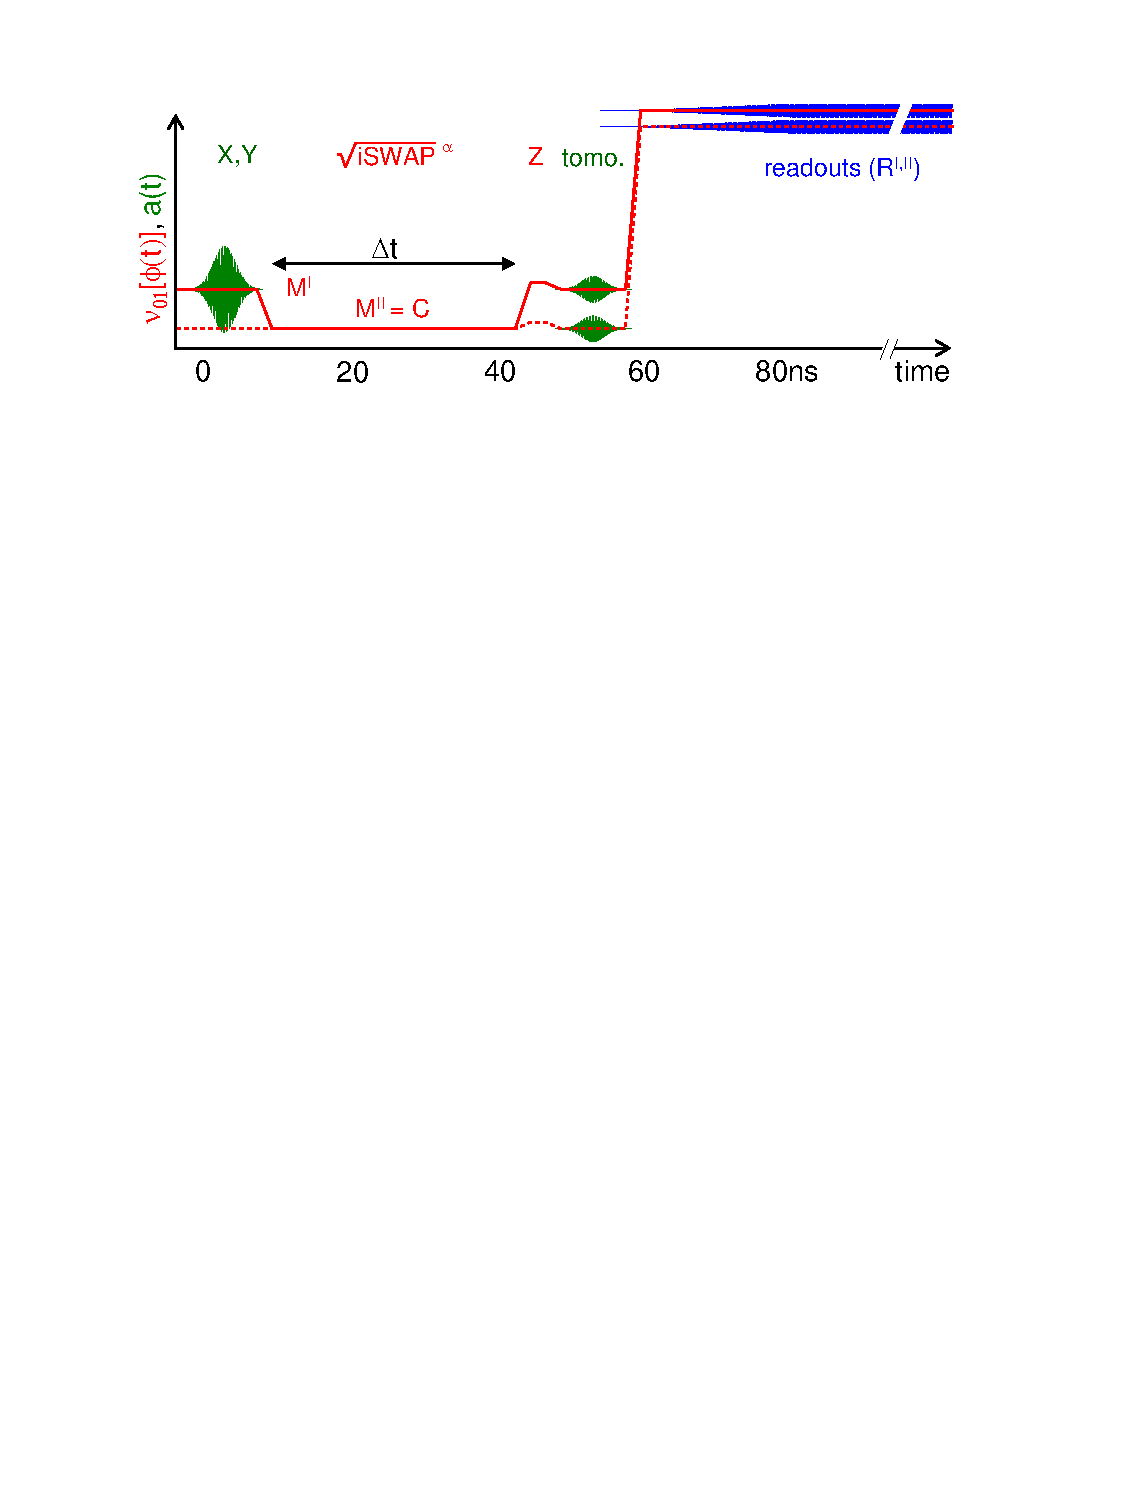
\includegraphics[width=0.8\textwidth]{./material/papers/iswap/figures/iswap_gate_pulse_sequence}
	\label{fig:ISwapPulseSequence}
	\caption{}
\end{figure}

\subsubsection{Violation of Bell's inequality}

\begin{figure}
	\centering
		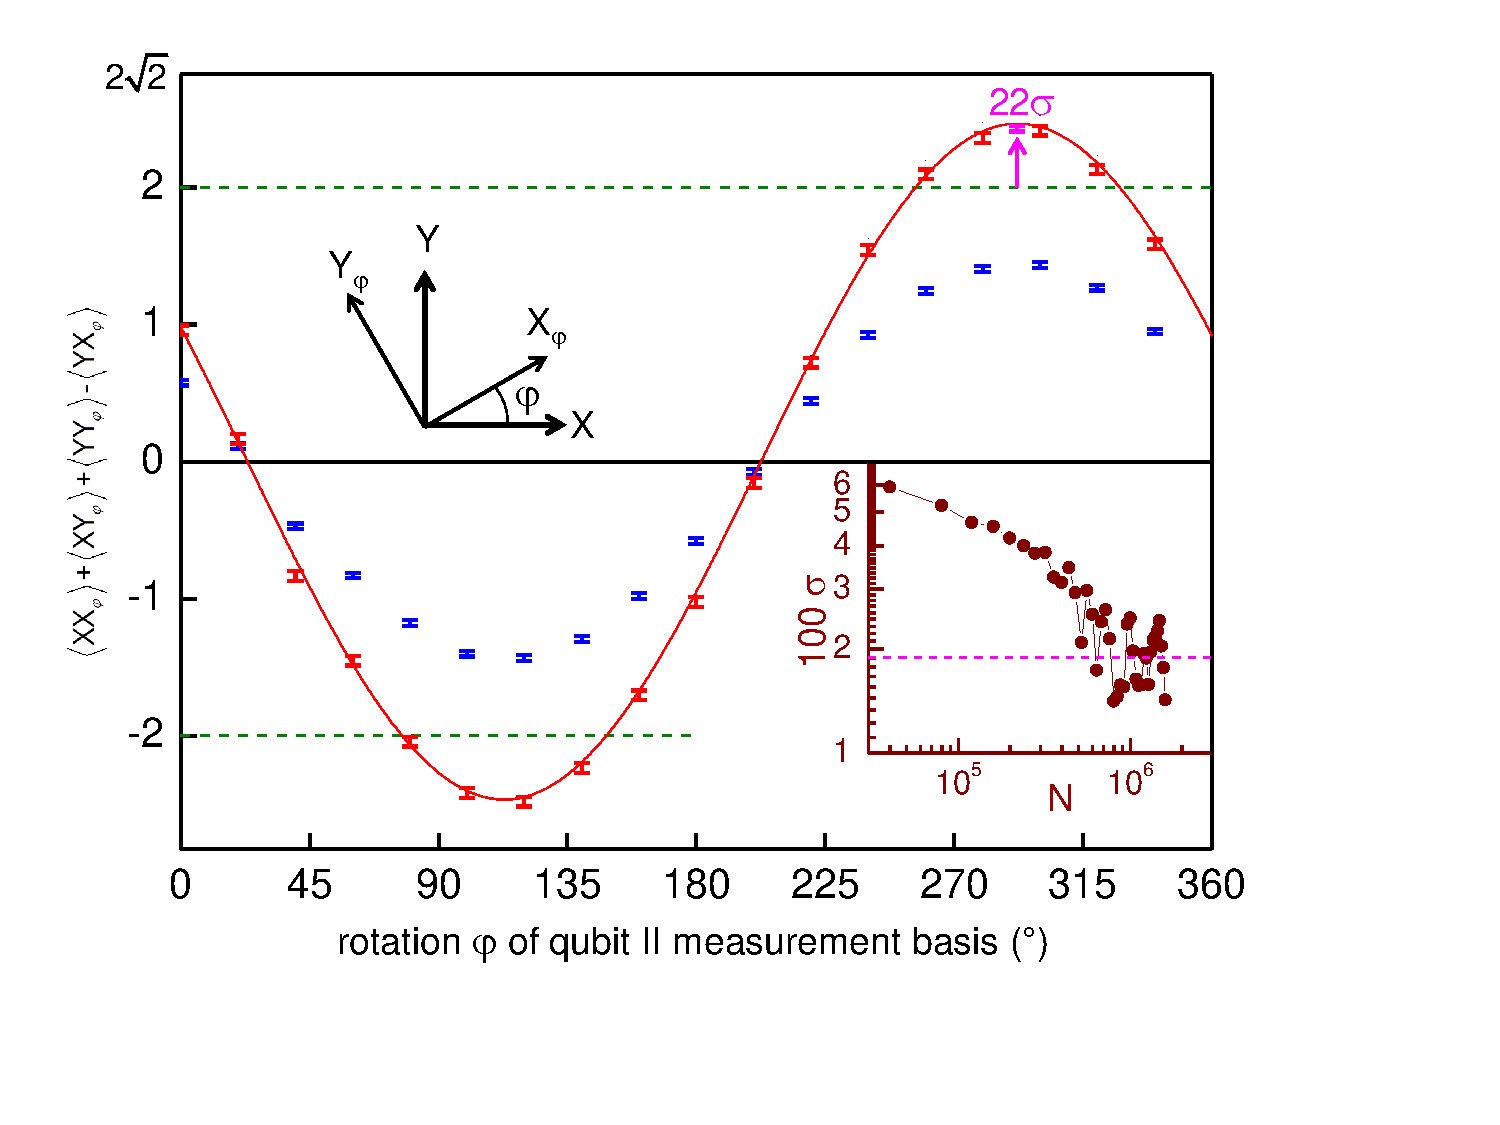
\includegraphics[width=0.8\textwidth]{./material/papers/iswap/figures/chsh}
	\label{fig:CHSH}
	\caption{}
\end{figure}

\subsection{Characterizing Quantum Processes}

\subsubsection{Introduction \& Principle}

\subsubsection{Implementation}

A quantum process can be described as a map $\mathcal{E} : \rho_\mathcal{H} \to \rho_\mathcal{H}$ that maps a density matrix $\rho$ defined in a Hilbert space $Q_1$ to another density matrix $\mathcal{E}(\rho)$ defined in a target Hilbert space $Q_2$ and fulfilling three axiomatic properties \cite{michael_a._nielsen_quantum_2000,haroche_exploring_2006}:

\begin{axiom}
$\mathrm{tr}\left[\mathcal{E}(\rho)\right]$ is the probability that the process represented by $\mathcal{E}$ occurs, when $\rho$ is the initial state.
\end{axiom}

\begin{axiom}
$\mathcal{E}$ is a {\it convex-linear map} on the set of density matrices, that is, for probabilities $\left\{p_i\right\}$,

  \begin{equation}
	  \mathcal{E}\left(\sum\limits_i p_i \rho_i\right) = \sum\limits_i p_i \mathcal{E}(\rho_i)
	\end{equation}
\end{axiom}

\begin{axiom}
$\mathcal{E}$ is a {\it completely-positive} map. That is, if $\mathcal{E}$  maps density operators of system $Q_1$ to density operators of system $Q_2$, then $\mathcal{E}(A)$ must be positive for any positive operator $A$. Furthermore, if we introduce an extra system $R$ of arbitrary dimensionality, it must be true that $(\mathcal{I}\otimes \mathcal{E})(A)$ is positive for any positive operator $A$ on the combined system $RQ_1$, where $\mathcal{I}$ denotes the identity map on system $R$.
\end{axiom}
As shown in \cite{michael_a._nielsen_quantum_2000}, any quantum process fulfilling these criteria can be written in the form

\begin{equation}
  \mathcal{E}(\rho) = \sum\limits_i E_i \rho E_i^\dagger \label{eq:process_operator_sum_representation}
\end{equation}
for some set of operators $\{ E_i \}$ which map the input Hilbert space to the output Hilbert space, and $\sum_i E_i^\dagger E_i \le I$.

Now, if we express the operators $E_i$ in a different operator basis $\tilde{E}_j$ such that $E_i = \sum_j a_{ij} \tilde{E}_{j}$ and insert into eq. (\ref{eq:process_operator_sum_representation}), we obtain

\begin{eqnarray}
 \mathcal{E}(\rho) & = & \sum\limits_i \sum\limits_j a_{ij} \tilde{E}_j \;\rho\; \sum\limits_k a_{ik}^* \tilde{E}_k^\dagger \\
& = & \sum\limits_{j,k}\tilde{E}_j \; \rho \; \tilde{E}_k^\dagger \sum\limits_i a_{ij} a_{ik}^* \\
& = & \sum\limits_{j,k}\tilde{E}_j \; \rho \; \tilde{E}_k^\dagger \; \chi_{jk} \label{eq:process_chi_representation}
\end{eqnarray}
where we defined $\chi_{jk} = \sum\limits_i a_{ij} a_{ik}^*$. This is the so-called $\chi$-matrix representation of the quantum process. Here, all the information on the process is contained in the $\chi$ matrix, which controls the action of the process-independent operators $\tilde{E}_i$ on the initial density matrix $\rho$.

Now, the goal of {\it quantum process tomography} is to obtain the coefficients of the $\chi$-matrix -- or any other complete representation of the process -- from a set of experimentally measured density matrices $\rho$ and $\mathcal{E}(\rho)$.

To achieve this, several techniques have been developed. The technique used in this work is the so-called {\it standard quantum process tomography (SQPT)}. This technique proceeds as follows:

\begin{enumerate}
\item Choose a set of operators $E_i$ that forms a full basis of $\mathcal{M}: Q_1 \to Q_2$. For n-qubit process tomography we usually choose $E_{i_1,i_2 \hdots i_n} = \sigma_{i_1}\otimes \sigma_{i_2}\hdots\otimes\sigma_{i_n}$, where $\sigma_i$ are the single-qubit Pauli operators and $i\in\{I,X,Y,Z\}$. 
\item Choose a set of pure quantum states $\ket{\phi_i}$ such that $\ket{\phi_i}\bra{\phi_i}$ span the whole space of input density matrices $\rho$. Usually, for a n-qubit system we choose $\phi = \{\ket{0},\ket{1},(\ket{0}+\ket{1})/\sqrt{2},(\ket{0}+i\ket{1})/\sqrt{2}\}^{\otimes n}$, where $^{\otimes n}$ denotes the n-dimensional Kronecker product of all possible permutations.
\item For each of the $\ket{\phi_i}$, determine $\mathcal{E}(\ket{\phi_i}\bra{\phi_i})$ by quantum state tomography. Usually we also determine $\ket{\phi_i}\bra{\phi_i}$ experimentally since the preparation of this state already entails small preparation errors that should be taken into account when performing quantum process tomography. 
\end{enumerate}

After having obtained the $\rho_i$ and $\mathcal{E}(\rho_i)$ one obtains the $\chi$-matrix by writing $\mathcal{E}(\rho_i) = \sum_j \lambda_{ij} \tilde{\rho}_j$, with some arbitrary basis $\tilde{\rho}_j$ and
letting $\tilde{E}_m \tilde{\rho}_j \tilde{E}_n^\dagger = \sum_k \beta_{jk}^{mn}\tilde{\rho}_k$. We can then insert into eq. (\ref{eq:process_chi_representation}) and obtain
\begin{eqnarray}
\sum\limits_k \lambda_{ik} \tilde{\rho}_k & = & \sum\limits_{m,n} \chi_{mn} \sum\limits_k \beta_{ik}^{mn} \tilde{\rho}_k  
\end{eqnarray}
This directly yields $\lambda_{ik} = \sum_{m,n}\beta_{ik}^{mn}\; \chi_{mn}$, which, by linear inversion,  gives $\chi$.

\subsubsection{The Kraus representation}

Besides the $\chi$-matrix representation, there is another useful way of expressing a quantum map, the so called {\it Kraus representation}, which is given as

\begin{equation}
 \mathcal{E}(\rho) = \sum\limits_i M_i \; \rho \; M_i^\dagger \label{eq:process_kraus_representation}
\end{equation}

It can be shown \citep{haroche_exploring_2006} that this sum contains at most $N$ elements, where $N$ is the dimension of the Hilbert space of the density matrix $\rho$. We can go from the $\chi$ representation to the Kraus representation by changing the basis $\tilde{E}_i$ such that

\begin{equation}
	\tilde{E}_i = \sum\limits_l a_{il}\; \breve{E}_l
\end{equation}

which, for eq. (\ref{eq:process_chi_representation}), yields

\begin{eqnarray}
 \mathcal{E}(\rho) & = & \sum\limits_{j,k} \sum\limits_l a_{jl} \breve{E}_l \; \rho \sum\limits_m a_{km}^* \breve{E}_m^\dagger \; \chi_{jk} \\
 & = & \sum\limits_{l,m}  \breve{E}_l \; \rho \; \breve{E}_m^\dagger \; \sum\limits_{j,k} a_{jl} a_{km}^* \chi_{jk} \label{eq:process_chi_transformed}
\end{eqnarray}

The last sum on the right side of eq. (\ref{eq:process_chi_transformed}) corresponds to a change of coordinates of the matrix $\chi$. Now, we can pick the $a$ such that $\chi$ is diagonal in the new basis $\breve{E}$ and obtain

\begin{eqnarray}
 \mathcal{E}(\rho) & = &  \sum\limits_{l} \lambda_l \breve{E}_l \; \rho \; \breve{E}_l^\dagger \\
& = &  \sum\limits_{l} M_l \; \rho \; M_l^\dagger
\end{eqnarray}
with $\lambda_l$ being the $l$-th eigenvalue of the $\chi$ matrix with the eigen-operator $\breve{E}_l$ and $M_{l} = \sqrt{\lambda_l} \breve{E}_l$.


\subsection{Realizing a Two-Qubit Gate}

\begin{figure}
   \centering
	 \includegraphics[width=1.\textwidth]{"./data/ct5/film of swap/pauli_set_vs_time_with_simulation"}
	 \caption[test]{testcaption}
	 \label{fig:swap_pauli_set_vs_time_with_simulation}
\end{figure}

\subsubsection{Principle}

\subsubsection{Implementation}

\subsubsection{Fidelity}

\subsubsection{Error Analysis}

%-Discuss the realization of a 2 qubit gate:
%  -Principle
%  -Implementation & Pulse Sequency
%  -Characterization through Quantum Process Tomography:
%     -Principles: State tomography, Pauli set, process tomography
%     -Discuss alternative representations of the process information:
%        -Chi matrix, Choi matrix, S, log S, Kraus operator representation
%  		-Errors: Discuss simulations, error models and possible reasons for discrepancies

\begin{figure}
	\centering
		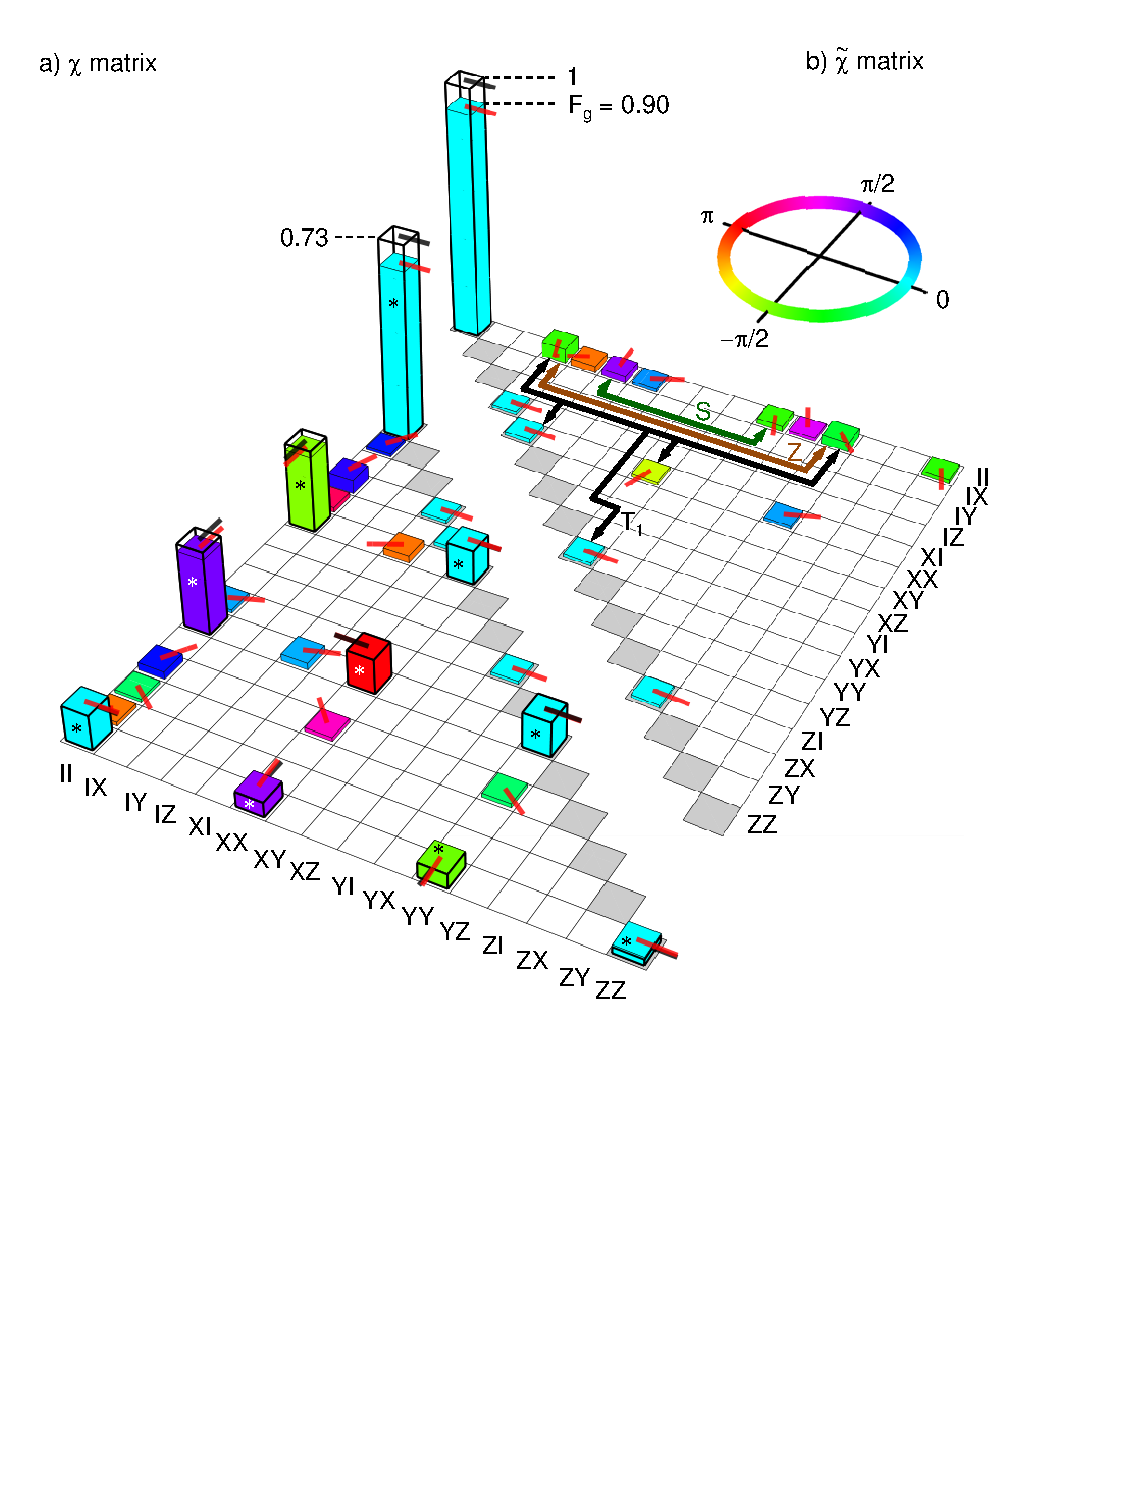
\includegraphics[width=1.\textwidth]{./material/papers/iswap/figures/chi_matrix_and_error_process}
	\label{fig:GateChiMatrixAndErrorProcess}
	\caption{}
\end{figure}


\section{Running Grover's Search Algorithm}

%Motivate this experiment:
% -Benchmark for superconducting quantum computers
% -Speed-up for searching in an unsorted database

\begin{figure}
	\centering
		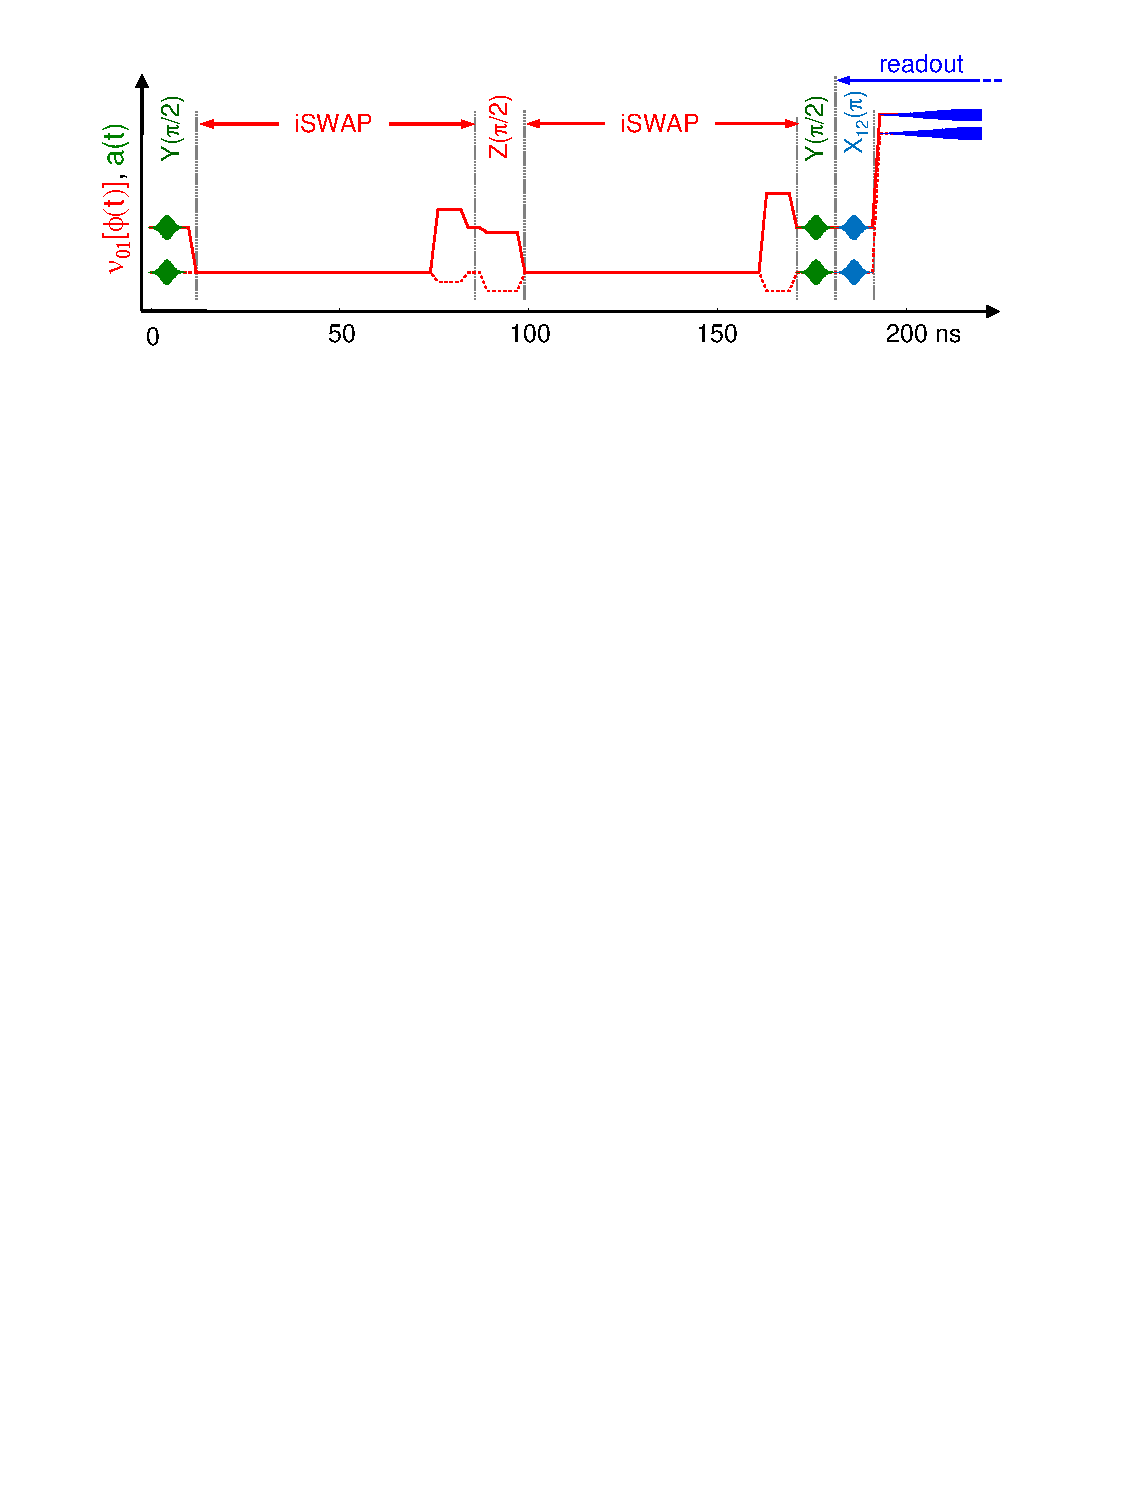
\includegraphics[width=1.\textwidth]{./material/papers/grover/figures/grover_algorithm_pulse_sequence}
	\label{fig:Grover3}
	\caption[Pulse sequence used for implementing Grovers search algorithm]{The pulse sequence used in realizing Grover's quantum search algorithm. First, a $Y_{\pi/2}$ pulse is applied to each qubit to produce the fully superposed state $1/2(\ket{00}+\ket{01}+\ket{10}+\ket{11})$. Then, an $i\mathrm{SWAP}$ gate is applied, followed by a $Z_{\pm \pi /2}$ gate on each qubit, which corrsponds to the application of the oracle function. The resulting state is then analyzed using another $i\mathrm{SWAP}$ gate and two $Y_{\pi/2}$ gates to extract the state which has been marked by the oracle function. Optionally, a $Y^{12}_{\pi}$ pulse is used on each qubit to increase the readout fidelity.}
\end{figure}

\subsection{Introduction \& Motivation}

\begin{enumerate}
  \item {\textbf Inputs:} An oracle function $\mathcal{O}$ which performs the operation $O\ket{x}\ket{q} = \ket{x}\ket{q\otimes f(x)}$, where $f(x) = \delta_{x,x_0}$
  \item {\textbf Outputs:} The marked state $x_0$
	\item Initialize the qubit register to the state: 
	$$\ket{\psi} \to \ket{0}^{\otimes n}\ket{0}$$
	\item Apply the Hadamard transformation to all of the qubits: 
	$$\ket{psi}\to \frac{1}{\sqrt{2^n}}\sum\limits_{x=0}^{2^n-1} \ket{x} \left[ \frac{\ket{0}-\ket{1}}{\sqrt{2}} \right]$$
	\item Apply the Grover iteration $R \approx [\pi \sqrt{2^n}/4]$ times:
	$$ \ket{\psi} \to \left[(2 \ket{\psi}\bra{\psi}-I)\mathcal{O}\right]^R \frac{1}{\sqrt{2^n}} \sum\limits_{x=0}^{2^n-1}\ket{x} \left[ \frac{\ket{0}-\ket{1}}{\sqrt{2}} \right] \approx \ket{x_0}\left[\frac{\ket{0}-\ket{1}}{\sqrt{2}}\right] $$
	\item Measure the first n qubits to obtain $x_0$
\end{enumerate}

For the Two-qubit case, this algorithm can be drastically simplified -- or ``compiled'' -- such that it runs without the ancilla qubit and in one single step of the Grover iteration:

\begin{enumerate}
  \item {\textbf Inputs:} An oracle function $\mathcal{O}$ which performs the operation $O\ket{x} =(-1)^{\delta_{x,x_0}}\ket{x}$, where $x_0$ is the marked state that is searched.
  \item {\textbf Outputs:} The marked state $x_0$
	\item 
\end{enumerate}

%-Explain the Grover experiment...
%		-Theoretical interest
%		-First demonstration in NMR
%   -Potential speed-up
%   -Details of the algorithm:
%     -Elementary operations
%     -Pulse shapes, corrections, ...

\begin{figure}
	\centering
		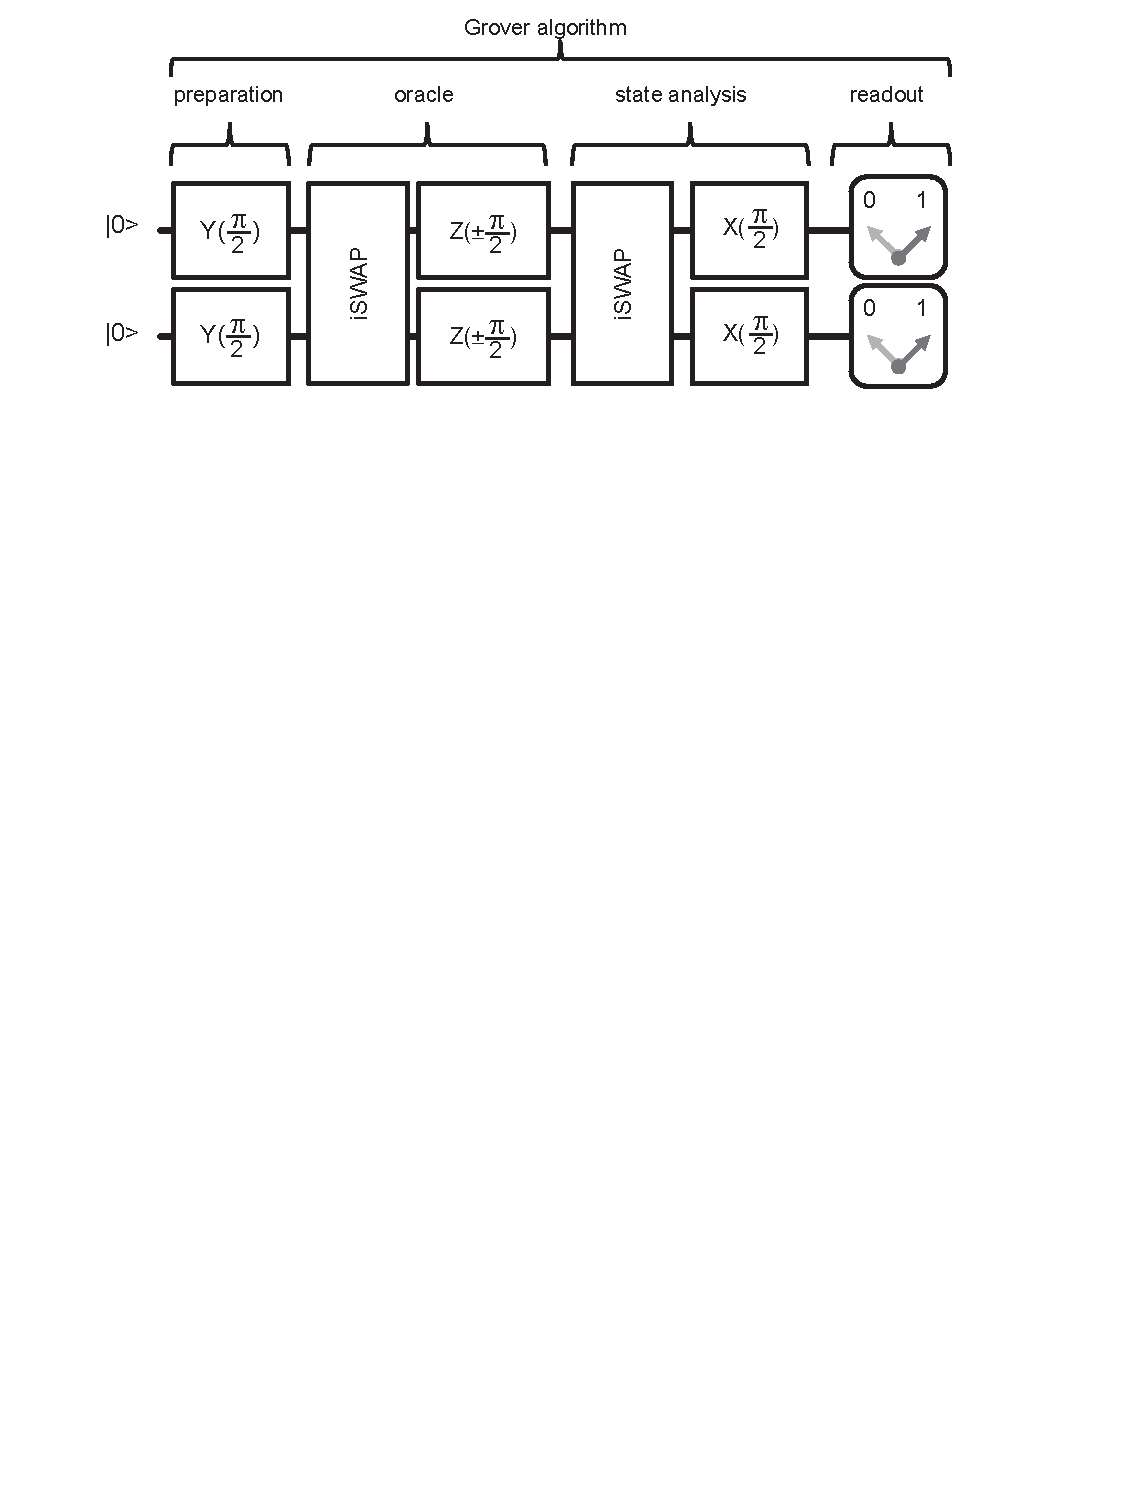
\includegraphics[width=1.\textwidth]{./material/papers/grover/figures/grover_algorithm_schematic}
	\label{fig:GroverAlgorithmSchematic}
	\caption{}
\end{figure}

\subsection{Experimental Implementation}

%-Show the implementation principle of the experiment.
%  -Break down the algorithm using the universal quantum gates that we've implemented

\subsection{Results}

%To Do:
%  -Create figures for all steps of the algorithm using Matplotlib
%  -Re-Analyze the data using Denis' Mathematica
%-Discuss the results and errors.

\begin{figure}
	\centering
		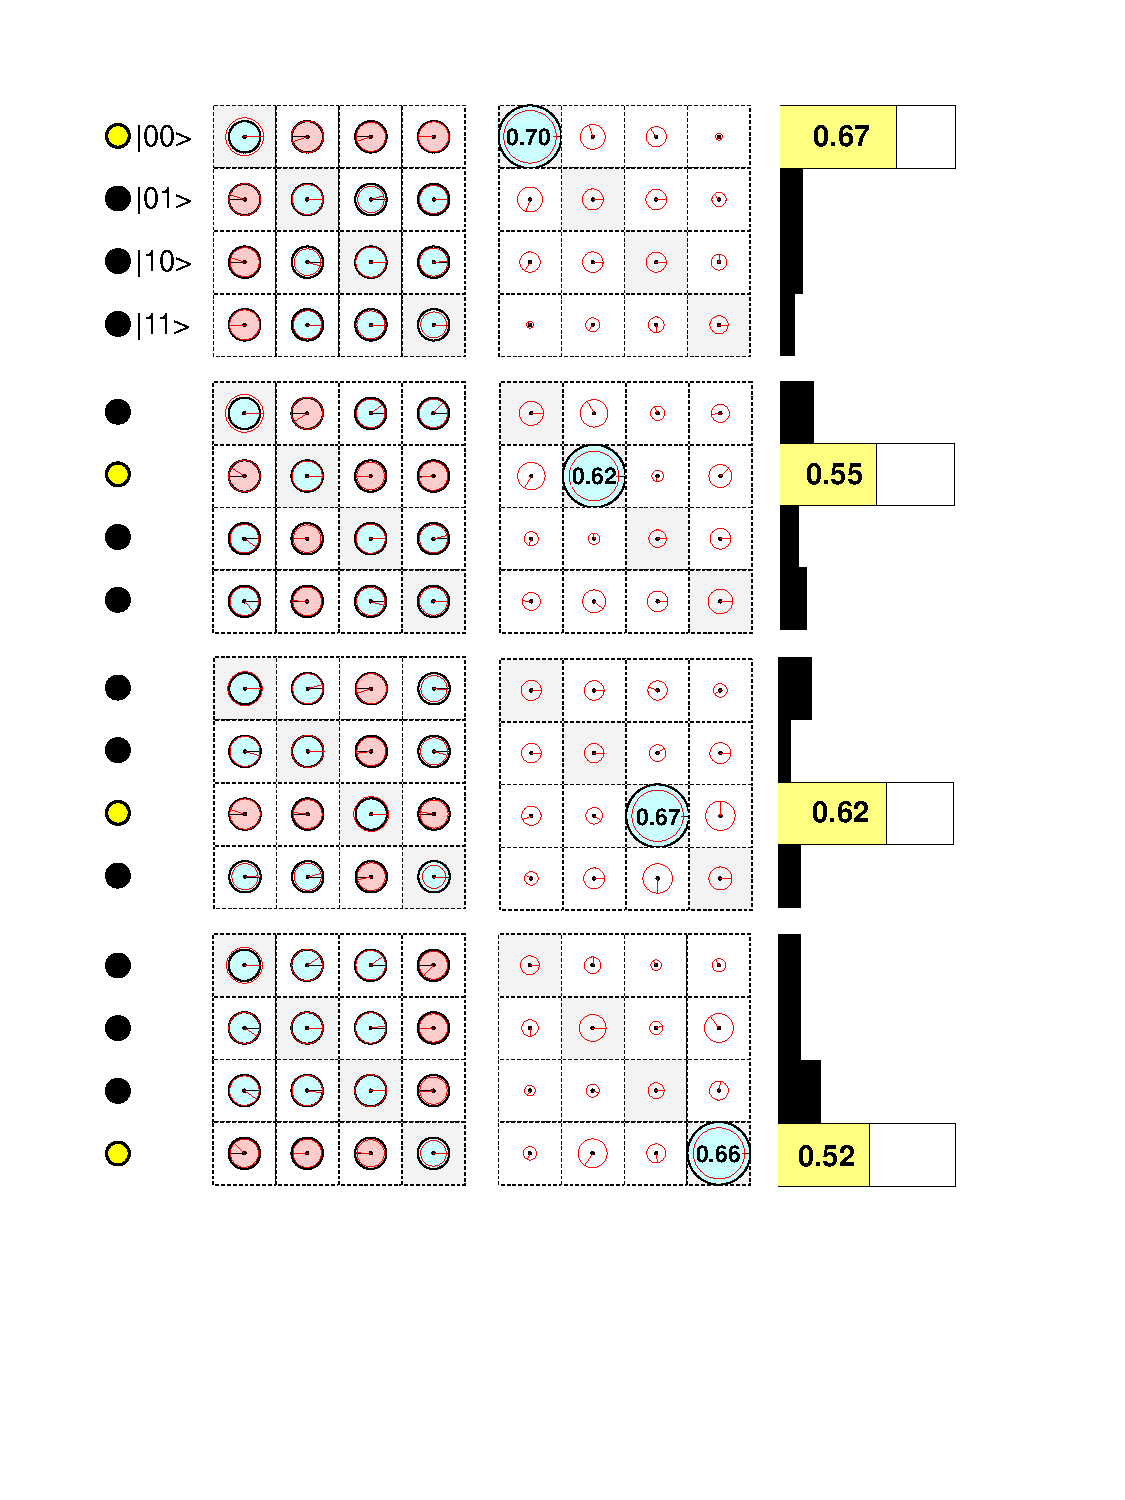
\includegraphics[width=1.\textwidth]{./material/papers/grover/figures/grover_algorithm_experimental_results}
	\label{fig:GroverAlgorithmExperimentalResults}
	\caption{}
\end{figure}

\subsubsection{Algorithm Fidelity}


\subsubsection{Single-Run Probabilities}

\subsubsection{Error Analysis}

\subsection{Conclusions}

%-Conclusions regarding quantum speed-up and applicability of results to larger-scale quantum computing.
